\documentclass[a4paper,12pt]{report}
\usepackage{times}
\usepackage{graphicx}
\usepackage[a4paper,
bindingoffset=0.2in,
left=1in,
right=.5in,
top=.7in,
bottom=.5in,
footskip=.25in]{geometry}
\usepackage{pdfpages}
\begin{document}
	\begin{center}
		\textbf{NETACODE -A SOFTWARE COMPANY VISITING REPORT}\\
		\begin{flushleft}
			The report is visiting a software company for \textbf{Course tittle:Information System Design with industrial attachment Sessional} Course and \textbf{Course Code:CSE 3210} in Computer Science and Engineering.\\
		\end{flushleft}
				by\\	
			Mst.Habiba Hena Sumi(200101070)\\Most.Jannat-Ul-Ferdoush(200101068)\\Md.Talath Un Nabi(200101076)\\Ferdous Tahsin(200101079)\\
			
			\begin{figure}[h]
				\centering
				\includegraphics[width=0.4\linewidth]{"images (1)"}
				\label{fig:images-1}
			\end{figure}
		
		\vspace{1 cm}
			Submited To:\\
			Teacher name:Ananna Hoque Shathi\\
			Department of Computer Science and Engineering(CSE)\\
			Bangladesh Army University of Science and Technology(BAUST)\\
			
		\end{center}
	
	\begin{flushright}
		\vspace{3 cm}
		...............................................\\
		signature of the teacher
	\end{flushright}
\newpage
\tableofcontents
\listoffigures
\newpage

\chapter{Systems Concepts and the Information Systems Environment}
\section{INTRODUCTION}
 System analysis and design is a process that many companies use to evaluate particular business situations and develop ways to improve them through more optimal methods.\\
 
\begin{figure}[h]
	\centering
	
\includegraphics[width=0.9\linewidth]{1_1}
	\label{fig:11}
\end{figure}

 Since 2019 ECNHOST LLC, Registered in Delaware, to provide fully managed reliable, scalable, and
 secure vps hosting solutions for individuals and businesses of all sizes . Netacode pride theirselves on solid
 network reliability and responsive 24/7 customer service. their cost-effective web hosting is suitable for
 establishing a Web presence or a website that requires the deployment and maintenance of fully
 integrated e-business solutions.
\section{NetaCode goal}
Netacode goal is simple and one that combines creativity with the latest research and development in the tech
world.they are a very customer-oriented company, putting our customers first and always focusing on
gaining and deserving the trust of every single one of their customers. So, they listen to their customers, stay
at the cutting edge of the latest trends in tech research, and constantly develop better web hosting
products and services which enable them to fulfill this vision better and better every day.
\\
\\

To provide trouble-free, customer-focused, reliable, and affordable web hosting services. they simply want
to continue to operate a profitable web hosting company that makes customers happy. Since the
beginning, they have backed they rock solid hosting solutions and top-notch infrastructure with the best
customer service and technical support. A common feeling about the technology field is it's all about
machines, yes, It does take machines but, Host Pair also knows it takes good people to run a well-oiled
machine. Yes, a successful business needs to be committed to client solutions, innovation, creativity, and
a warm, caring attitude to all of our customers' business needs. We don't just provide 24x7 support. they
really do listen and care.
\section {Characteristic of System:}
\textbf{Organization}
Their organization has a branch in Dinajpur district. Netacode is a multinational software company. Main office in Dhaka in Bangladesh. Their organizations are certainly very beautiful. 4 storied building and their number of rooms is 7.\\

\textbf{Interaction}
It is defined by the manner in which the components operate with each other.For example, in an organization,purchasing department must interact with production department and payroll with personnel department.\\

\textbf{Interdependence}
Interdependence means how the components of a system depend on one another. For proper functioning, the components are coordinated and linked together according to a specified plan. \\

\textbf{Integration}
Integration is concerned with how a system components are connected together. It means that the parts of the system work together within the system even if each part performs a unique function.\\

\textbf{Central Objective}
The objective of system must be central. It may be real or stated. It is not uncommon for an organization to state an objective and operate to achieve another.\\
\begin{figure}[h]
	\centering
	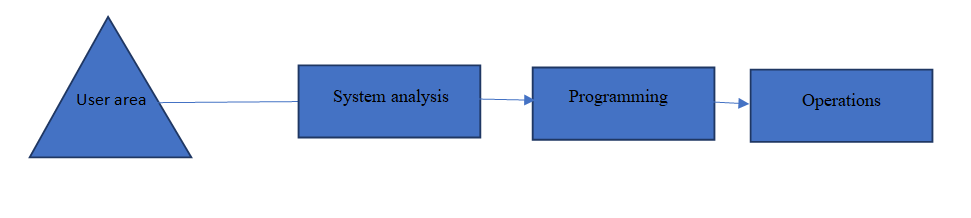
\includegraphics[width=0.7\linewidth]{1}
	\caption{Task Interdependence in a Computer – Based Subsystem }
	\label{fig:1}
\end{figure}
\section{Elements of System}
\textbf{Outputs and Inputs}
\begin{itemize}
	\item 	The main aim of a system is to produce an output which is useful for its user.
	\item 	Inputs are the information that enters into the system for processing.
	\item 	Output is the outcome of processing.
\end{itemize}
\textbf{Processor(s)}
\begin{itemize}
	\item 	The processor is the element of a system that involves the actual transformation of input into output.
	\item 	It is the operational component of a system. Processors may modify the input either totally or partially, depending on the output specification.
\end{itemize}
\textbf{control}
\begin{itemize}
	\item The control element guides the system.
	\item	It is the decision–making subsystem that controls the pattern of activities governing input, processing, and output.
\end{itemize}
\textbf{Feedback}
\begin{itemize}
	\item Feedback provides the control in a dynamic system.
	\item	Positive feedback is routine in nature that encourages the performance of the system.
	\item	Negative feedback is informational in nature that provides the controller with information for action.
\end{itemize}
\textbf{Environment}
\begin{itemize}
	\item	The environment is the “supersystem” within which an organization operates.
	\item	It is the source of external elements that strike on the system.
\end{itemize}
\textbf{Boundaries and Interface}
\begin{itemize}
	\item	A system should be defined by its boundaries. Boundaries are the limits that identify its components, processes, and interrelationship when it interfaces with another system.
	\item	Each system has boundaries that determine its sphere of influence and control.
\end{itemize}
\begin{figure}[h]
	\centering
	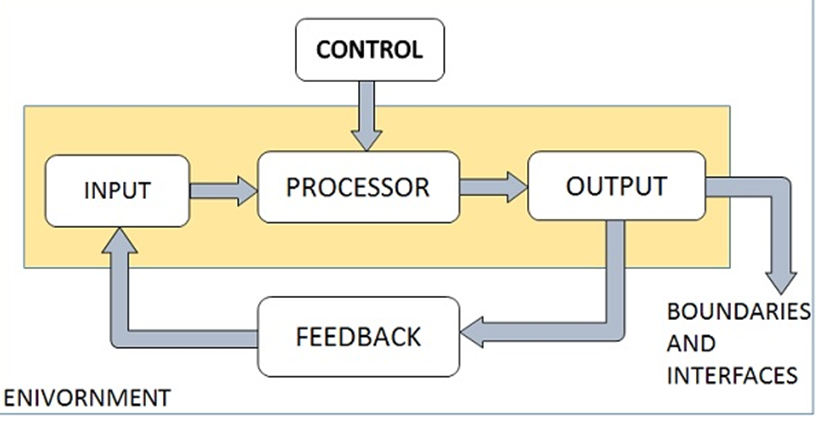
\includegraphics[width=0.7\linewidth]{2}
	\label{fig:2}
\end{figure}
\section{Types of Systems}
The systems can be divided into the following types 
\textbf{Physical or Abstract Systems}
\begin{itemize}
	\item	Physical systems are tangible entities. We can touch and feel them.
	\item	Physical System may be static or dynamic in nature. For example, desks and chairs are the physical parts of computer center which are static. A programmed computer is a dynamic system in which programs, data, and applications can change according to the user's needs.
	\item	Abstract systems are non-physical entities or conceptual that may be formulas, representation or model of a real system.
\end{itemize}
\textbf{Open or Closed Systems}
\begin{itemize}
	\item	An open system must interact with its environment. It receives inputs from and delivers outputs to the outside of the system. For example, an information system which must adapt to the changing environmental conditions.
	\item	A closed system does not interact with its environment. It is isolated from environmental influences. A completely closed system is rare in reality.
\end{itemize}
\begin{figure}[h]
	\centering
	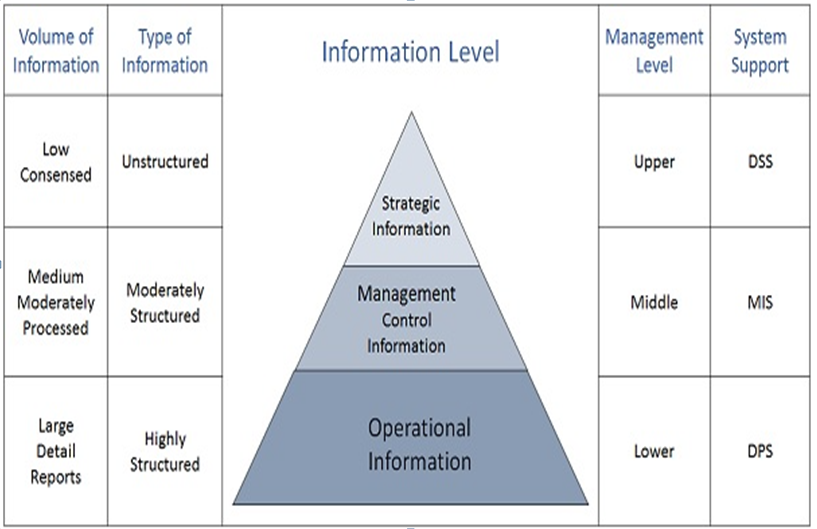
\includegraphics[width=0.7\linewidth]{3}
	\caption{Categories of information related to managerial levels and the decision managers make.}
	\label{fig:3}
\end{figure}
\textbf{Goals}\\
To provide trouble-free, customer-focused, reliable, and affordable web hosting services. WE simply want
to continue to operate a profitable web hosting company that makes customers happy. \\Since the
beginning, we have backed our rock solid hosting solutions and top-notch infrastructure with the best
customer service and technical support. A common feeling about the technology field is it's all about
machines, yes, It does take machines but, Host Pair also knows it takes good people to run a well-oiled
machine. Yes, a successful business needs to be committed to client solutions, innovation, creativity, and
a warm, caring attitude to all of our customers' business needs. We don't just provide 24x7 support. We
really do listen and care.
\paragraph{Summary}
\begin{enumerate}
\item In this article, we define the process of system analysis and design, outline the benefits of this process and list seven tools and techniques that may aid your organization in implementing its next system analysis and design process.
\item Systems analysts may serve as change agents who identify the organizational improvements needed, design systems to implement those changes, and train and motivate others to use the systems.
\item The analyst plays many roles, sometimes balancing several at the same time. The three primary roles of the systems analyst are: consultant, supporting expert, and agent of change."
\item The analyst is the key member of the Management Information System (MIS) and Decision Support System (DSS).
\end{enumerate}
\newpage
\chapter{The System Development Life Cycle }
\section{Introduction:}
The system development life cycle is a conceptual model used for project management that describes the stages involved in an information system development project,from an initial feasibility study through maintainence of the completed application. To understand system development,we need to recognize that a candidate system has a life cycle. The stages are shown below:
\begin{enumerate}
	\item Recognititon of need / initial investigation
	\item	Feasibility Study
	\item	Analysis
	\item Design
	\item	Implementation
	\item	Post-implementation and maintenance   
	\end{enumerate}
\begin{figure}[h]
	\centering
	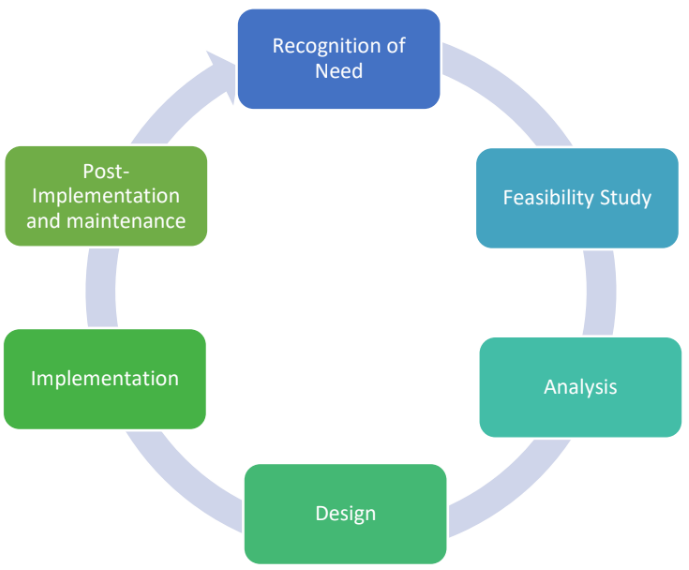
\includegraphics[width=0.7\linewidth]{2_1}
	\caption{System development life cycle}
	\label{fig:2_1}
\end{figure}
\section{Recognition of Need: }
One must know what the problems are before it can be solved. The basis for a candidate system is recognition of a need for improving an information system or a procedure. For example, a supervisor wants to investigate the system flow in purchasing.When we have completed our visit at netacode ,we discuss the recognition needs of their clients and how they collect and process the requirements to complete their project  successfully. They told us they have arranged meetings with their clients many times to understand and collect the requirements. They provide them forms and other documents to understand what is the actual need of their clients.If the problem is serious enough , management may want to have an analyst look at it. Such assignment  implies a commitment. At this stage only a rough estimation of the development cost of the project may be reached.If the problem is serious enough , management may want to have an analyst look at it. Such assignment  implies a commitment. At this stage only a rough estimation of the development cost of the project may be reached.
\section{Feasibility Study}
Depending on the initial investigation the survey expanded to a more detailed feasibility study. It is the test of a system proposal according to its workability. It focuses on three major questions:
\begin{enumerate}
	\item 	What are the users demonstrable needs and how does a candidate system meet them?
	\item	What resources are available for a given candidate system? Is the problem worth solving?
	\item	What are likely impacts of the candidate system on the organization? How does it fit within the organization MIS plan?
	\end{enumerate}
Each of these questions must be answered carefully. They revolved around the investigation and evaluation of the problem,identification and description of the candidate system,specification of performance and the cost of each system and final selection of the best system.\\ \\

The objective of the feasibility study is not to solve the problem but to acquire a sense of its scope. During the study the problem definition is crystalized and aspects of the problem to be included in the system are determined.\\ \\

The proposal summarizes what is known and what is going to be done. It is consist of the following:
\begin{enumerate}
	\item \textbf{Statement of the problem :} A carefully worded statement of the problem led to analysis.
	
	\item \textbf{	Summary of the findings and recommendations :} A list of the major findings and recommendations of the study. It is the idea for the user who requires quick access to the results of the analysis of the system under study. Conclusions are started followed by a list of the recommendations and a justification for them.
	
	\item \textbf{ Details of the findings :} an outline of the methods are procedures undertaken by the existing system,followed by coverage of the objectives and procedures of the candidate system. Included are also discussions of output reports, file structures, and cost and benefits of the candidate system.
	
	\item \textbf{	Recommendation and conclusions :} Specific recommendations regarding the candidate system, including personnel assignments, costs, project schedules and target dates.
\end{enumerate}
\section{Analysis:}
 It is the detailed study of the various operations performed by a system and their relationships within and outside of the system. A key question is : what must be done to solve the problem?\\ 
 
 When we visited the organization we discussed the analysis system. They first analys if they are able to complete it or not and then they discuss further processes that are steps they should take to make the project successful. Training, experience and common sense are required for collection of the information needed to do the analysis.
 \\ \\
 Once the analysis is completed, the analyst has a firm understanding what is to be done. The next step is to decide how the problem must be solved. Thus in system design, we move from the logical to physical aspects of the life cycle of a project.\\
 \section{Design:}
 The most creative and challenging phase of a system life cycle of a project is system design. The term design describes a final system and the process by which it is developed. It refers to the technical specifications that will be applied in implementing the project. The question is here: How should the problem be solved?\\
 
\begin{figure}[h]
	\centering
	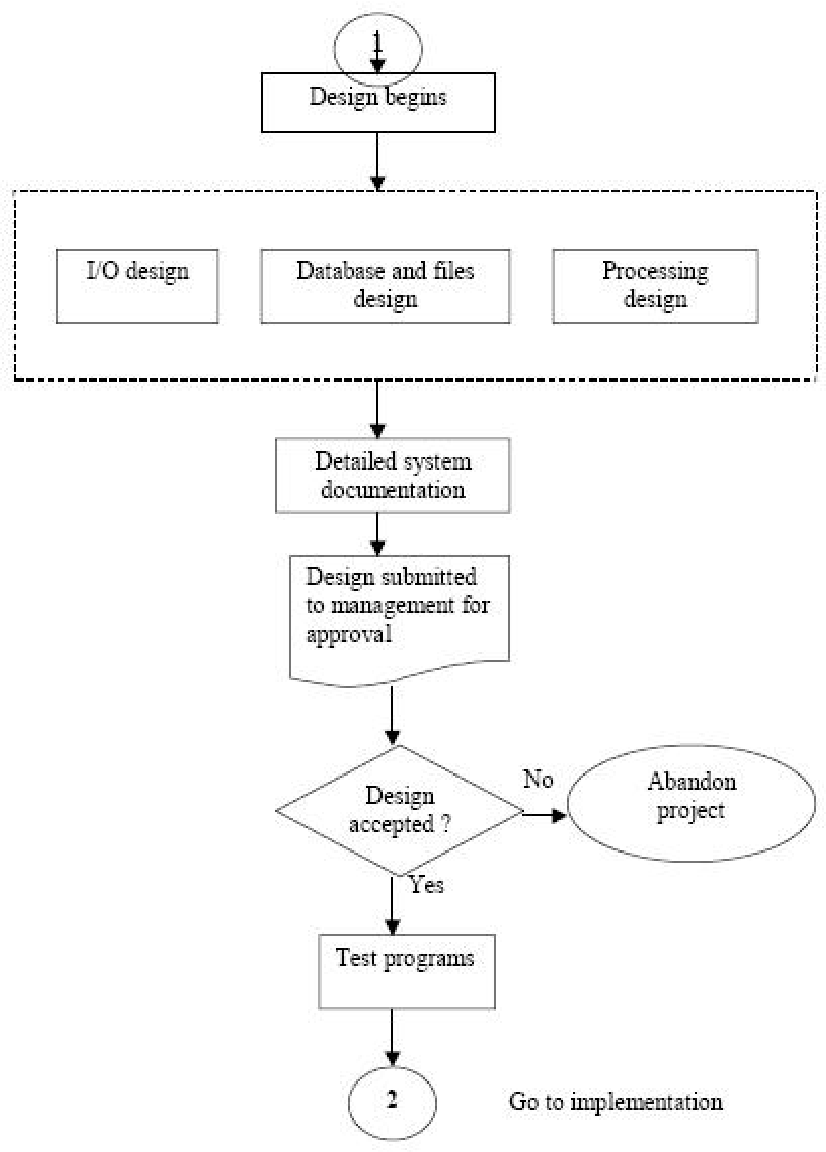
\includegraphics[width=0.7\linewidth]{fig-2;chap-2}
	\caption{design of a system}
	\label{fig:fig-2chap-2}
\end{figure}
The first step is to determine how the output is to be produced and in what form. Samples of the output are also presented. Second, input data and master files  are designed to meet the requirements of the proposed output. Finally details related to justification of the project and an estimate of the impact of the candidate system on the user and the organization  are documented and evaluated by management as a step toward implementation.
\\ \\
In netacode they first create a virtual design of the project by adobe illustrator or figma.then they present it to their clients to justify if it has been according to their requirements or not.\\
In some firms, separate groups of programmers do the programming , whereas other firms employ analyst programmers who do analysis.
\section{Implementation:}
The implementation sector is less creative than system design. It is primarily concerned with user training, site preparation and file conversion. Depending on the nature of the system, extensive user training may be required. Conversion usually takes place at about the same time the user is being trained or later.\\

In netacode they told us they used  react js as frontend development and node js for backend development. They also use nuxt js and next js for development. They used php but now they have shifted to javascript. \\

Once the program becomes available,test data is read into the computer and  processed against the file(s) provided for testing. If successful, the program(s) is then run with live data. Otherwise  a diagnostic procedure is used to locate and correct errors in the program. In most conversions a parallel run is conducted where the new system runs simultaneously with the old system. 
\section{Post termination and Maintenance : }
After the installation phase is completed and the user stuff is adjusted to the changes created by the candidate system, evaluation and  maintenance begin. Like any system, there is an aging process that requires periodic maintenance of hardware and software. If the new information is inconsistent with the design specifications, the changes have to be made. The importance of maintenance is to continue to bring the new system to standards.\\ 

The policy of Netacode is to serve their clients with the project they have created according to the requirements. but they don't share the source code of any project and if their updates are available, they do it take charges. This is their strategy of post implementation and maintenance of any project.
\paragraph{Summary}
\newpage
\chapter{The Role of the System Analyst}
\section{Introduction}
Systems analysts analyse how well software, hardware and the wider IT system fit the business needs of their employer or of a client. They write requirements for new systems and may also help implement them and monitor their effectiveness. Typical responsibilities of the job include: examining current systems.
\paragraph{System Analysis:} 
A person who conducts a methodical study and evaluation of an activity such as a business to identify its desired objective in order to determine procedurs by which these objectives can be gained.
\section{THE SYSTEMS ANALYST}
The systems analyst plays a key role in information systems development projects. The systems analyst works closely with all project team members so that the team develops the right system in an effective way. Systems analysts must understand how to apply technology to solve business problems. In addition, systems analysts may serve as change agents who identify the organizational improvements needed, design systems to implement those changes, and train and motivate others to use the systems.\\
\textbf{Netacode interpersonal skills relevant to systems work include the following: }\\
\textbf{Communication:}having the ability to articulate and speak the Jan guage of the user, a "flare" for mediation, and a knack for working with virtually all managerial levels in the organization Communication is not just reports, telephone conversations, and interviews, It is people talk ing, listening, feeling, and reacting to one another, their experience and reactions. Some indicators of a climate of closed communication are defensive memos, excessive correspondence, and a failure to speak up for fear of being identified. Therefore, opening communication channels are a must for system development.\\  \\
\textbf{Understanding}identifying problems and assessing their ramifications, having a grasp of company goals and objectives, and showing sensitivity to the impact of the system on people at work.
Teaching-educating people in use of computer systems, selling the system to the user, and giving support when needed. Selling-selling ideas and promoting innovations in problem solving using computers.
\subsection{Technical skills include:}
\textbf{Creativity}helping users model ideas into concrete plans and develop ing candidate systems to match user requirements.\\ \\
\textbf{Problem solving}reducing problems to their elemental levels for analy sis, developing alternative solutions to a given problem, and delineating the pros and cons of candidate systems\\ \\
\textbf{Project management}scheduling, performing well under time con straints, coordinating teain efforts, and managing costs and expendi **\\ \\
\textbf{Dynamite interface}blending technical and nontechnical consitlerastions in functional specifications and general design\\ \\
\underline{\textbf{NetacodeInterpersonal and Technical skill necessary in system Development :}}

\begin{figure}[h]
	\centering
	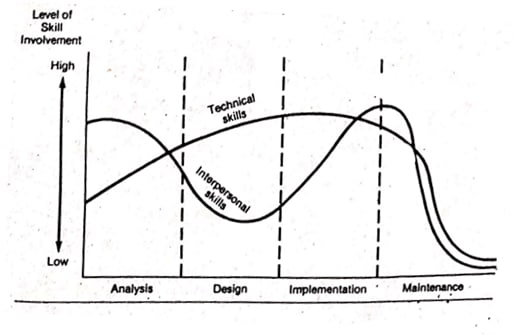
\includegraphics[width=0.9\linewidth]{3_1}
	\caption{Interpersonal and Technical Skills}
	\label{fig:31}
\end{figure}
\section{The background and experience of analysts include:}
\begin{enumerate}
	\item Abackground in systems theory and organization behavior. 
	\item  Familiarity with the makeup and inner workings of major application areas such as financial accounting, personnel administration, market ing and sales, operations management, model building, and production control.
	\item  Competence in system tools and methotlologies and a practical knowledge of one or more programming and data base languages. Experience in hardware and software specifications, which is important for selection.
\end{enumerate}
\section{The attributes are:}
\textbf{Authority-}the confidence to "tell" people what to do. Much of this quality shows in project management and team work to meet deadlines. Communication skills-ability to articulate and focus on a problem area for logical solution.\\
\textbf{Creativity-}trying one's own ideas, developing candidate systems using unique tools or methods.\\
\textbf{Hesponsibility-}making decisions on one's own and accepting the conequences of these decisions.\\
\textbf{Varied skills-}doing different projects and handling change.
\paragraph{Summary }
\begin{enumerate}
	\item A systems analyst is a person who conducts a study, identifies activities and objectives, and determines a procedure to achieve the objectives. Systems analysis has a history dating back to Taylor. Early analysts worked in factories, specializing in improving work methods and set ting time standards for production. With the advent of the computer. the analyst asstimed the role of a problem solver and a specialist m developing computer applications.
	\item Success in systems analysis requires interpersonal and technical skills Interpersonal skills emphasize communication and interface with the user, whereas technical skills include creativity, problem solving, and managing the overall project. During analysis, there is greater need for interpersonal skills, but during design there is greater emphasis on technical skills. During implementation, both skills are needed
	\item A career in systems analysis requires academic preparation, experience, and good interpersonal relations. The person must be familiar with the inner-workings of business and competent in system tools and meth odologies. The personal qualities include creativity and communications skills and being systematic and sensitive.
	\item Analysts perform a multitude of roles-as change agent, investigator. architect. psychologist salesperson, and motivator They also need to understand politics.
\end{enumerate}
\chapter{Systems Planning and the Initial Investigation}
\section{Bases for planning in system analysis :}
It is a systematic approach, which uses graphical tools that analyze and refine the objectives of an existing system and develop a new system specification which can be easily understandable by user. It has following attributes: It is graphic which specifies the presentation of application.
\section{Strategic MIS Planning}
Planning for information system development must be done within the framework of the Netacodeoverall MIS plan. The time horizon dimension specifics whether it is short. which is tantamount to the MIS yearly plan medium term , or long range. The focus dimension tells whether the primary concern is strategic, managerial, or operational strategic (MIS) planning is an orderly approach that determines the basic objectives for the user to achieve, the strategies and policies needed to achieve the objectives, and the tactical plans to implement the strategies. The first task in strategic planning is to set the MIS objectives and the results expected. Consideration of these objectives must deal with their fit with the organization's strategic plan, the types of systems and services to be offered, the role of users in system development, and the technology to be used. 
Managerial and Operational MTS Planning Managerial MIS planning integrates strategic with operational plans. It is a process in which specific functional plans are related to specific number of years to show how strategies are to be carried out to achieve long-range plans. The next step is to devise short-range plans that spell out the day-to-day activities of the system. They are programmed plans requiring a year's commitment. For example, the operating expense budget, the human resource budget of each computer application, and timetables for implementing a new system are all short-range plans designed to implement the organization's master plan by computerizing the labor-intensive areas of the business.
\section{Strategies for Determining Information Requirements}
There are three key strategies or general approaches for eliciting information regarding the user's requirements:
\begin{enumerate}
	\item asking, \item Getting information from the existing information system, and \item Prototyping 
\end{enumerate}
\paragraph{Asking} This strategy obtains information from users by simply ask. ing them about the requirements. It assumes a stable system where users are well informed and can overcome biases in defining their problem.There are three key asking methods:
\begin{enumerate}
	\item Questions may be open-ended or closed. An open-ended question allows the respondent to formulate a response. It is used when feelings or opinions are important. For example, "How do you evaluate the latest addition to your hardware?" In contrast, a closed question requests one answer from a specific set of responses. It is used when factual responses are known. 
	\item Brainstorming is a technique used for generating new ideas and obtaining general information requirements. This method is appropriate for eliciting nonconventional solutions to problems, A guided approach to brainstorming asks each participant to define ideal solutions and then select the best feasible one. 
	\item Group consensus asks participants for their expectations regarding specific variables a Delphi inquiry. for example, each participant fills out a questionnaire The results are  summarized and given to participants along with a follow up questionnaire. Participants are invited to change their responses. The results are again summarized and fed back to the participants. This debate by questionnaire continues until participants responses have converged enough. This method has an advantage over brainstorming in that participants are not subjected to psychological pres sure from others with presumed authority or influence.	
\end{enumerate}
\paragraph{Summary}
\begin{enumerate}
	\item Planning information systems has become increasingly important be cause information is a vital resource and company asset, more and more funds are committed to information systems, and system develop ment is a serious business for computers that incorporate data bases and networking
	\item Planning for information systems has a time horizon and a focus di mensionThe time horizon dimension specifics the time range of the plan, whereas the forus dimension relates whether the primary con cem is strategic, managenal, or operational.
	\item The initial investigation has the objective of determining the validity of the user's request for a candidate system and whether a feasibility study should be conducted. The objectives of the problem posed by the user must be understood within the framework of the organization's MIS plan
	\item Detemming user requirements is not easy. System requirements change, the articulation of requirements is difficult, and heavy user involvement and motivation are uncertain. Problems with the user analyst interface add further dilliculties to the procedure.
	\item There are three strategies for eliciting information regarding the user's requirements asking questions, obtaining information from the juvent system, and juntotyping. The asking strategy assumes a stable system when the user is well informed about information requirements. In contrast the prototyping strategy is appropriate for high-un ertainty.
\end{enumerate}
\chapter{Information Gathering}
\section{Introduction}
Information is stimuli that has meaning in some context for its receiver. When information is entered into and stored in a computer, it is generally referred to as data. After processing -- such as formatting and printing -- output data can again be perceived as information. When information is compiled or used to better understand something or to do something, it becomes knowledge.
\section{How Netacode collects information from clients.}
\begin{figure}[h]
	\centering
	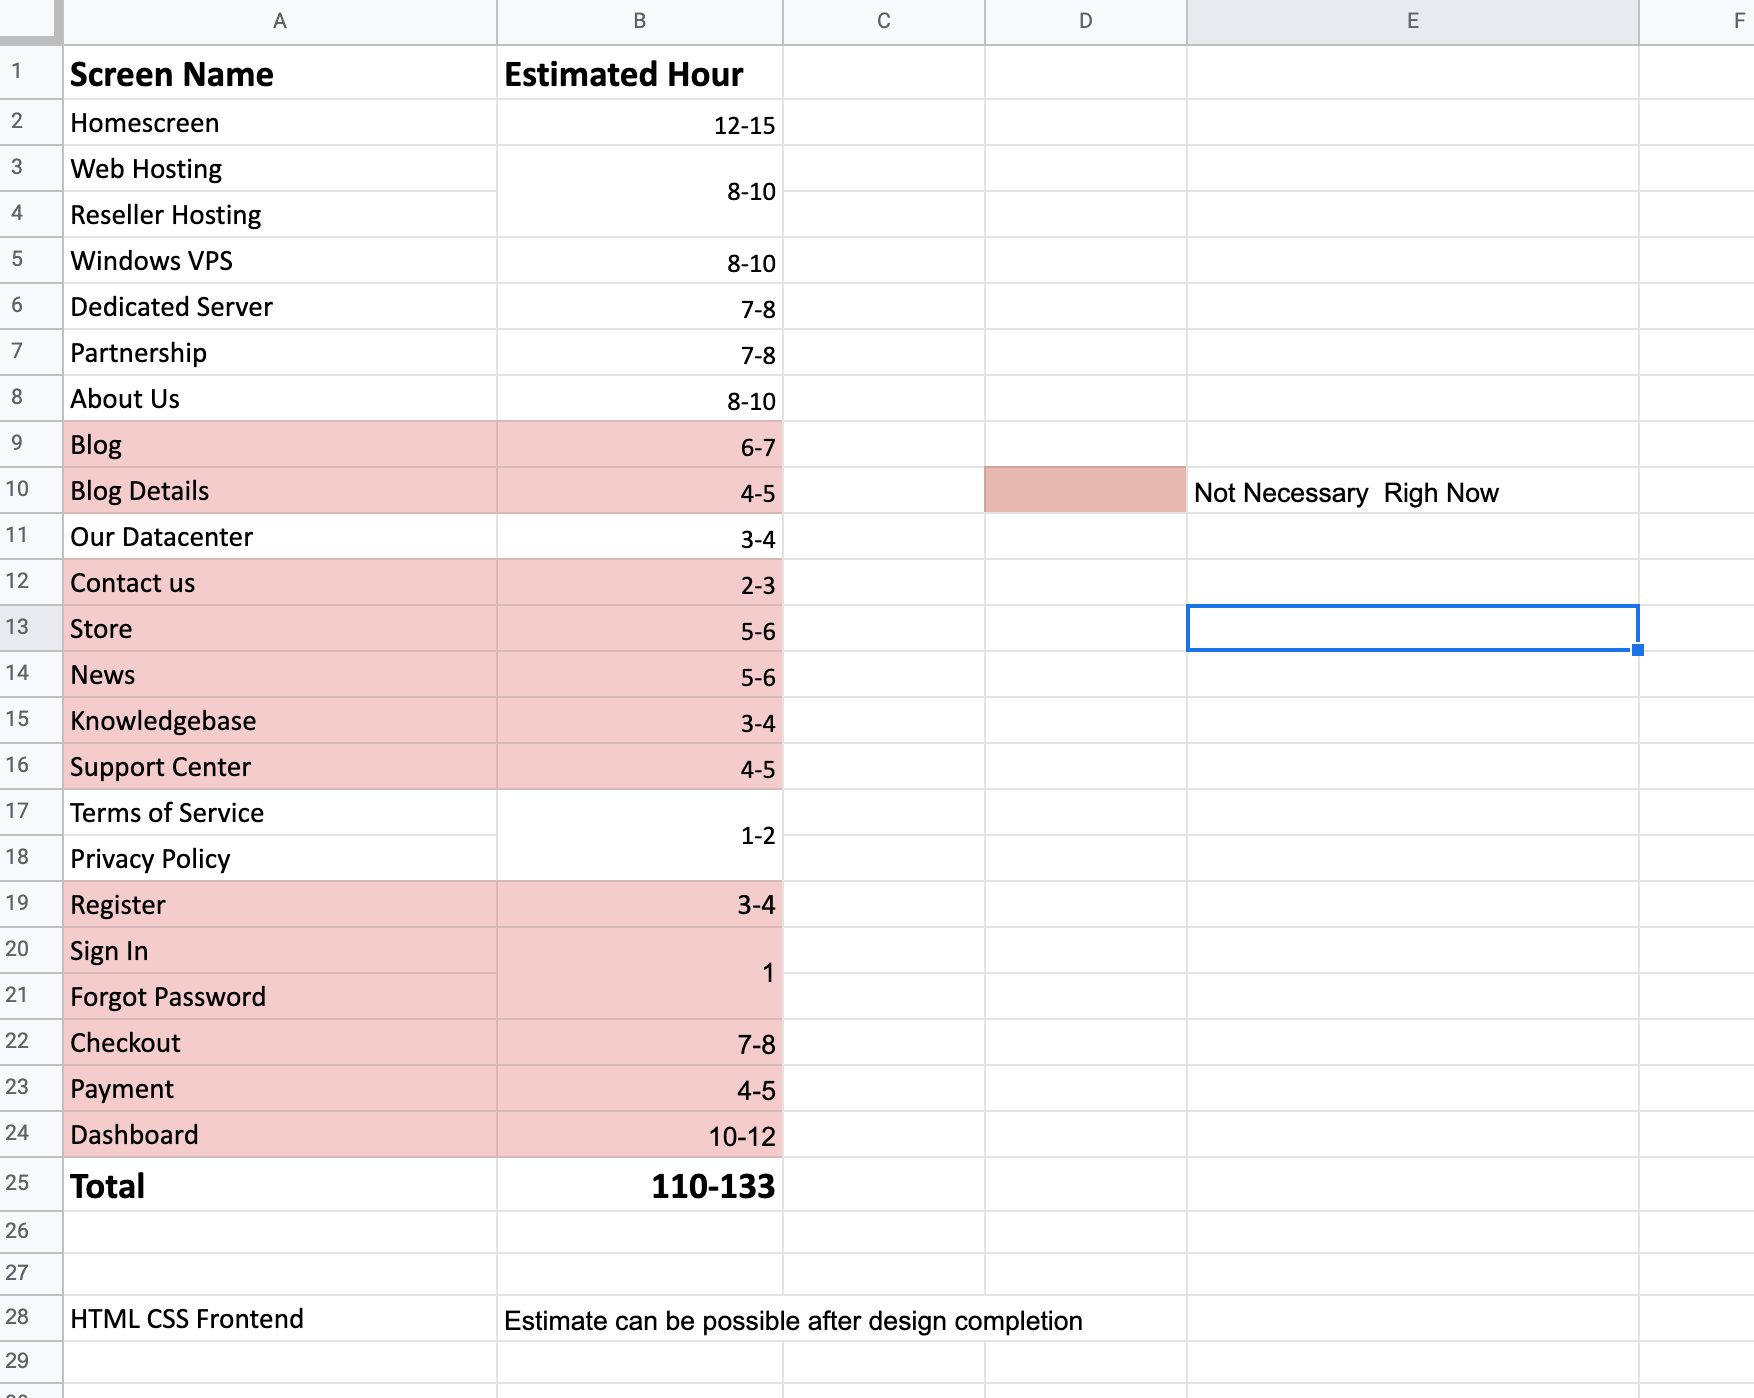
\includegraphics[width=0.7\linewidth]{5_1}
	\caption{Information Collection}
	\label{fig:51}
\end{figure}
Netacode uses various data collection tools to collect necessary information from clients. Then, they make project timeline according to the client's requirements. 
\section{Information about the firm}
The following Organization Chart for Netacode is displayed below.
\newpage
\begin{figure}[h]
	\centering
	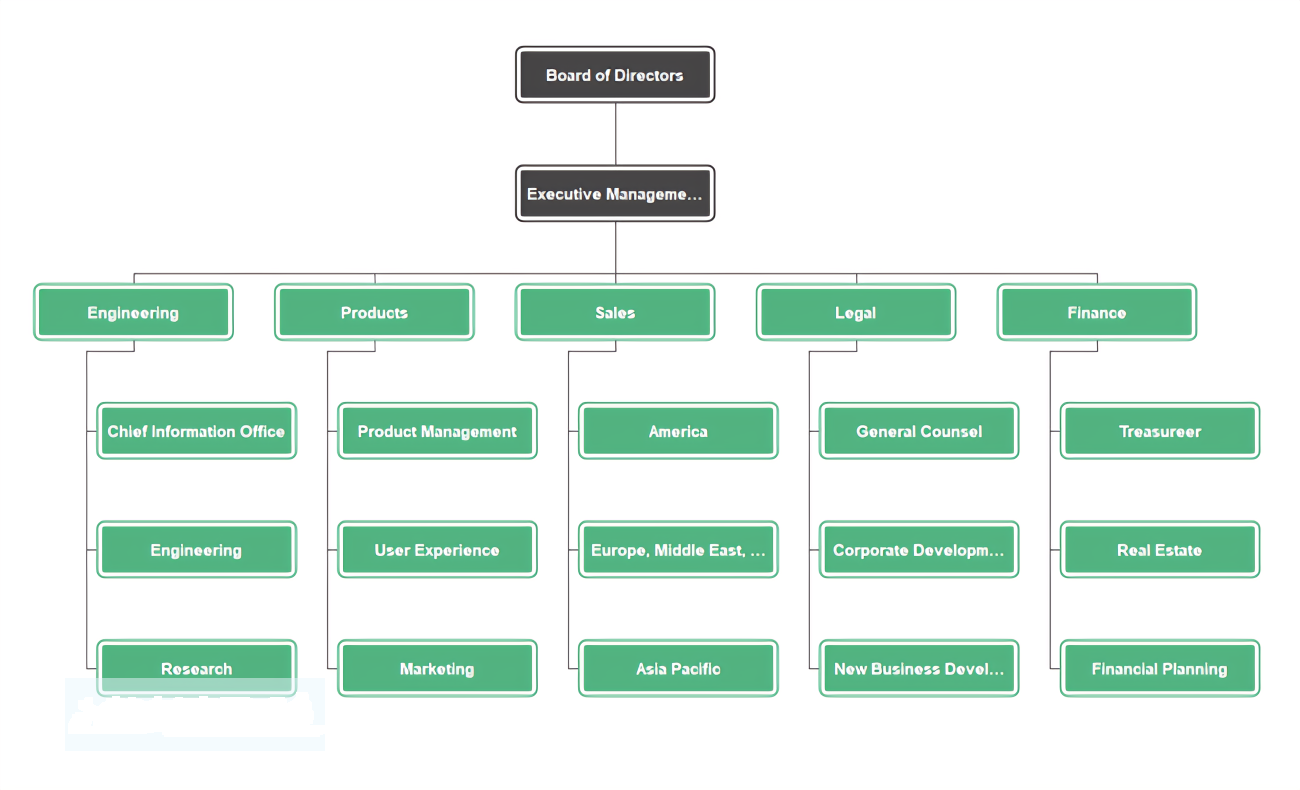
\includegraphics[width=0.9\linewidth]{5_2}
	\caption{Organization Chart of Netacode}
	\label{fig:52}
\end{figure}

\section{Information Gathering Method – Questionaries}
Since information must be acquired accurately, methodically, under the right conditions, and
with minimum interruption to user personnel there is some tools which have been used to gather
information. Though there are various kinds of information gathering tools we use:\\
\begin{enumerate}
	\item  Review of literature, procedures and forms.
	\item  On-site observation
	\item  Interviews
	\item Questionnaires
\end{enumerate}
In order to learn more about Netacode, we used a questionnaire form.
	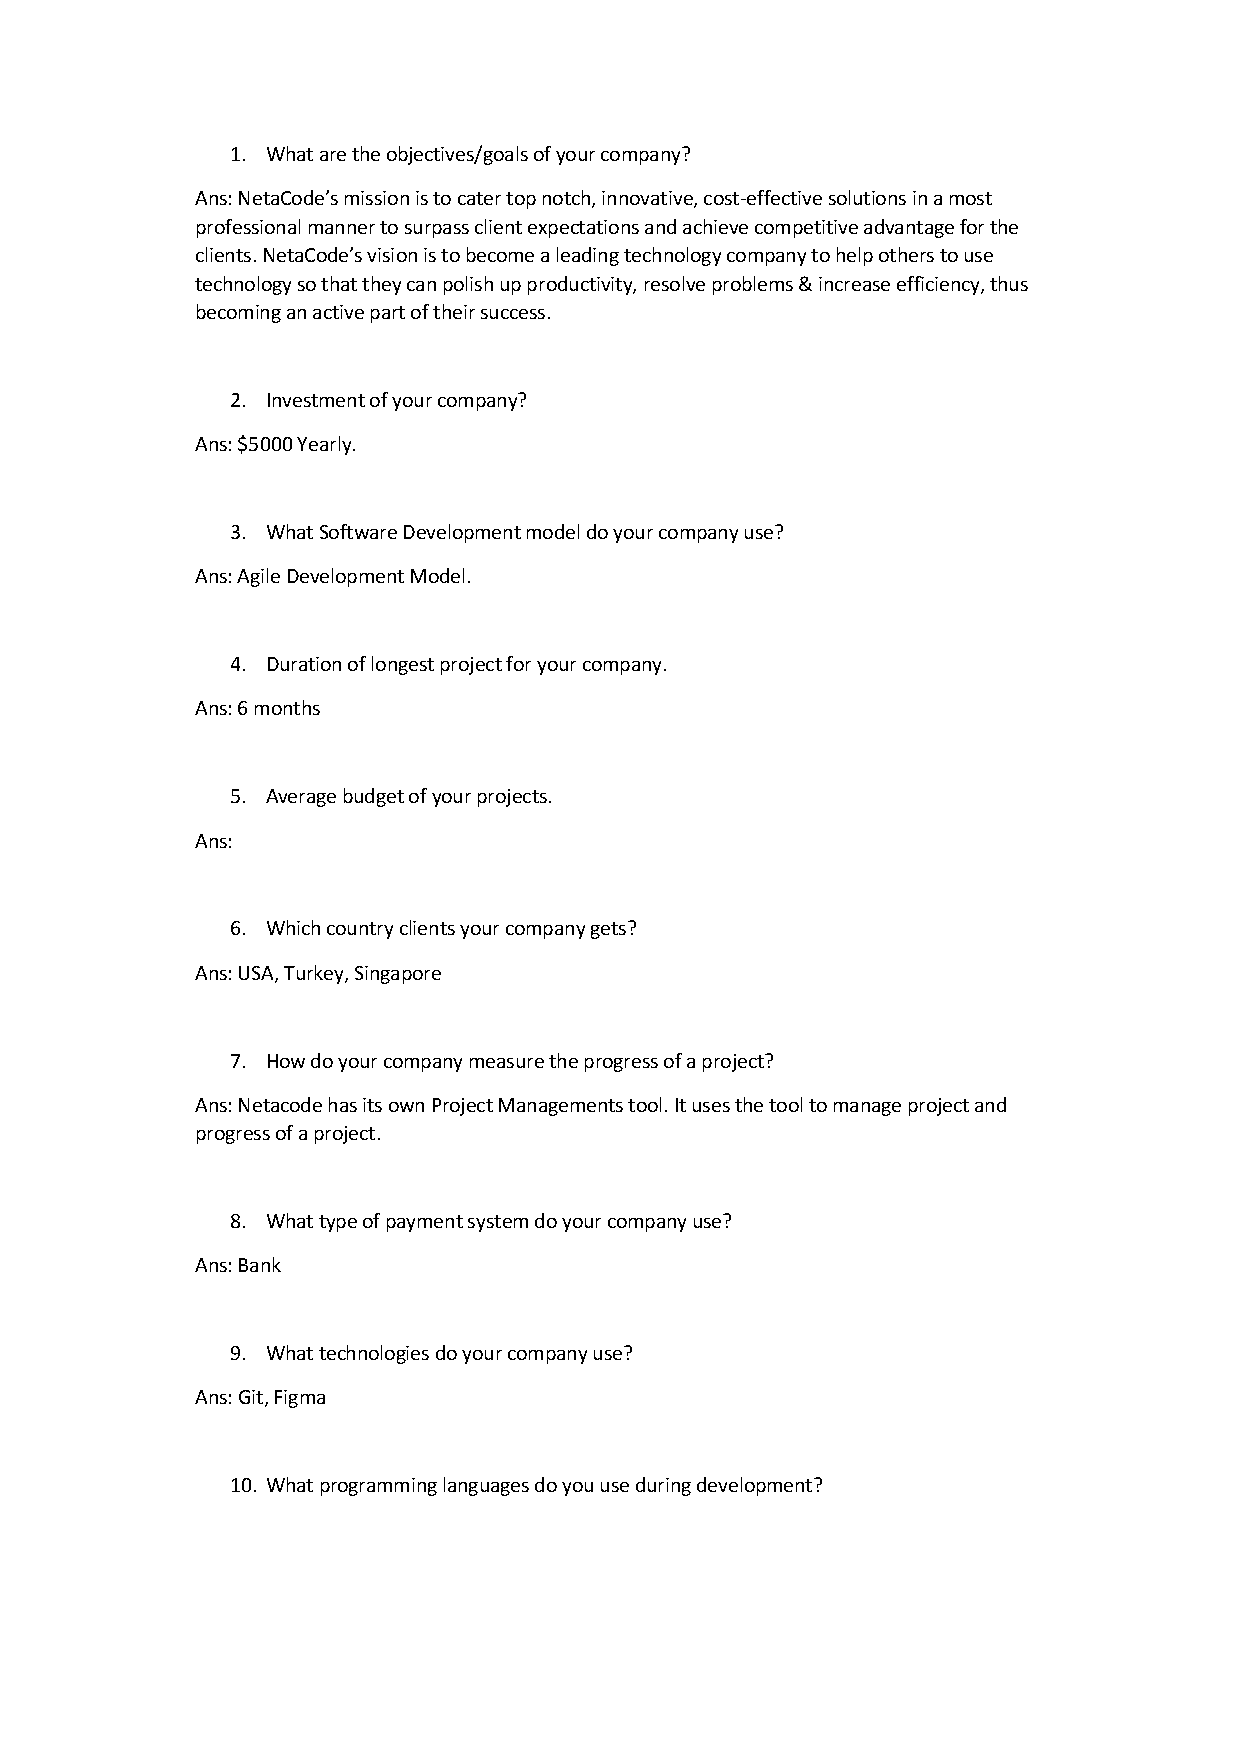
\includepdf[pages={1,2}] {5_question.pdf}
\paragraph{Conclusion}
This chapter taught us about numerous techniques for acquiring information as well as the Netacode company's organizational structure, which we visited. We also learned about the methods used by Netacode to gather client information.

\end{document}
